\documentclass[1p]{elsarticle_modified}
%\bibliographystyle{elsarticle-num}

%\usepackage[colorlinks]{hyperref}
%\usepackage{abbrmath_seonhwa} %\Abb, \Ascr, \Acal ,\Abf, \Afrak
\usepackage{amsfonts}
\usepackage{amssymb}
\usepackage{amsmath}
\usepackage{amsthm}
\usepackage{scalefnt}
\usepackage{amsbsy}
\usepackage{kotex}
\usepackage{caption}
\usepackage{subfig}
\usepackage{color}
\usepackage{graphicx}
\usepackage{xcolor} %% white, black, red, green, blue, cyan, magenta, yellow
\usepackage{float}
\usepackage{setspace}
\usepackage{hyperref}

\usepackage{tikz}
\usetikzlibrary{arrows}

\usepackage{multirow}
\usepackage{array} % fixed length table
\usepackage{hhline}

%%%%%%%%%%%%%%%%%%%%%
\makeatletter
\renewcommand*\env@matrix[1][\arraystretch]{%
	\edef\arraystretch{#1}%
	\hskip -\arraycolsep
	\let\@ifnextchar\new@ifnextchar
	\array{*\c@MaxMatrixCols c}}
\makeatother %https://tex.stackexchange.com/questions/14071/how-can-i-increase-the-line-spacing-in-a-matrix
%%%%%%%%%%%%%%%

\usepackage[normalem]{ulem}

\newcommand{\msout}[1]{\ifmmode\text{\sout{\ensuremath{#1}}}\else\sout{#1}\fi}
%SOURCE: \msout is \stkout macro in https://tex.stackexchange.com/questions/20609/strikeout-in-math-mode

\newcommand{\cancel}[1]{
	\ifmmode
	{\color{red}\msout{#1}}
	\else
	{\color{red}\sout{#1}}
	\fi
}

\newcommand{\add}[1]{
	{\color{blue}\uwave{#1}}
}

\newcommand{\replace}[2]{
	\ifmmode
	{\color{red}\msout{#1}}{\color{blue}\uwave{#2}}
	\else
	{\color{red}\sout{#1}}{\color{blue}\uwave{#2}}
	\fi
}

\newcommand{\Sol}{\mathcal{S}} %segment
\newcommand{\D}{D} %diagram
\newcommand{\A}{\mathcal{A}} %arc


%%%%%%%%%%%%%%%%%%%%%%%%%%%%%5 test

\def\sl{\operatorname{\textup{SL}}(2,\Cbb)}
\def\psl{\operatorname{\textup{PSL}}(2,\Cbb)}
\def\quan{\mkern 1mu \triangleright \mkern 1mu}

\theoremstyle{definition}
\newtheorem{thm}{Theorem}[section]
\newtheorem{prop}[thm]{Proposition}
\newtheorem{lem}[thm]{Lemma}
\newtheorem{ques}[thm]{Question}
\newtheorem{cor}[thm]{Corollary}
\newtheorem{defn}[thm]{Definition}
\newtheorem{exam}[thm]{Example}
\newtheorem{rmk}[thm]{Remark}
\newtheorem{alg}[thm]{Algorithm}

\newcommand{\I}{\sqrt{-1}}
\begin{document}

%\begin{frontmatter}
%
%\title{Boundary parabolic representations of knots up to 8 crossings}
%
%%% Group authors per affiliation:
%\author{Yunhi Cho} 
%\address{Department of Mathematics, University of Seoul, Seoul, Korea}
%\ead{yhcho@uos.ac.kr}
%
%
%\author{Seonhwa Kim} %\fnref{s_kim}}
%\address{Center for Geometry and Physics, Institute for Basic Science, Pohang, 37673, Korea}
%\ead{ryeona17@ibs.re.kr}
%
%\author{Hyuk Kim}
%\address{Department of Mathematical Sciences, Seoul National University, Seoul 08826, Korea}
%\ead{hyukkim@snu.ac.kr}
%
%\author{Seokbeom Yoon}
%\address{Department of Mathematical Sciences, Seoul National University, Seoul, 08826,  Korea}
%\ead{sbyoon15@snu.ac.kr}
%
%\begin{abstract}
%We find all boundary parabolic representation of knots up to 8 crossings.
%
%\end{abstract}
%\begin{keyword}
%    \MSC[2010] 57M25 
%\end{keyword}
%
%\end{frontmatter}

%\linenumbers
%\tableofcontents
%
\newcommand\colored[1]{\textcolor{white}{\rule[-0.35ex]{0.8em}{1.4ex}}\kern-0.8em\color{red} #1}%
%\newcommand\colored[1]{\textcolor{white}{ #1}\kern-2.17ex	\textcolor{white}{ #1}\kern-1.81ex	\textcolor{white}{ #1}\kern-2.15ex\color{red}#1	}

{\Large $\underline{12a_{0801}~(K12a_{0801})}$}

\setlength{\tabcolsep}{10pt}
\renewcommand{\arraystretch}{1.6}
\vspace{1cm}\begin{tabular}{m{100pt}>{\centering\arraybackslash}m{274pt}}
\multirow{5}{120pt}{
	\centering
	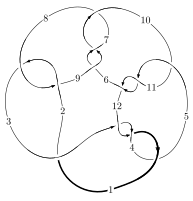
\includegraphics[width=112pt]{../../../GIT/diagram.site/Diagrams/png/1602_12a_0801.png}\\
\ \ \ A knot diagram\footnotemark}&
\allowdisplaybreaks
\textbf{Linearized knot diagam} \\
\cline{2-2}
 &
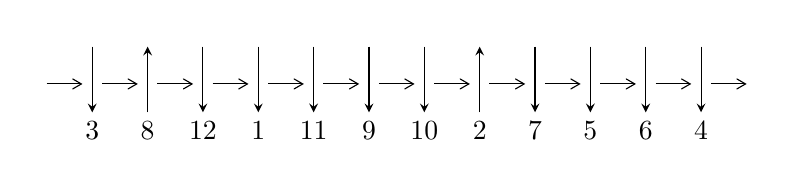
\begin{tikzpicture}[x=20pt, y=17pt]
	% nodes
	\node (C0) at (0, 0) {};
	\node (C1) at (1, 0) {};
	\node (C1U) at (1, +1) {};
	\node (C1D) at (1, -1) {3};

	\node (C2) at (2, 0) {};
	\node (C2U) at (2, +1) {};
	\node (C2D) at (2, -1) {8};

	\node (C3) at (3, 0) {};
	\node (C3U) at (3, +1) {};
	\node (C3D) at (3, -1) {12};

	\node (C4) at (4, 0) {};
	\node (C4U) at (4, +1) {};
	\node (C4D) at (4, -1) {1};

	\node (C5) at (5, 0) {};
	\node (C5U) at (5, +1) {};
	\node (C5D) at (5, -1) {11};

	\node (C6) at (6, 0) {};
	\node (C6U) at (6, +1) {};
	\node (C6D) at (6, -1) {9};

	\node (C7) at (7, 0) {};
	\node (C7U) at (7, +1) {};
	\node (C7D) at (7, -1) {10};

	\node (C8) at (8, 0) {};
	\node (C8U) at (8, +1) {};
	\node (C8D) at (8, -1) {2};

	\node (C9) at (9, 0) {};
	\node (C9U) at (9, +1) {};
	\node (C9D) at (9, -1) {7};

	\node (C10) at (10, 0) {};
	\node (C10U) at (10, +1) {};
	\node (C10D) at (10, -1) {5};

	\node (C11) at (11, 0) {};
	\node (C11U) at (11, +1) {};
	\node (C11D) at (11, -1) {6};

	\node (C12) at (12, 0) {};
	\node (C12U) at (12, +1) {};
	\node (C12D) at (12, -1) {4};
	\node (C13) at (13, 0) {};

	% arrows
	\draw[->,>={angle 60}]
	(C0) edge (C1) (C1) edge (C2) (C2) edge (C3) (C3) edge (C4) (C4) edge (C5) (C5) edge (C6) (C6) edge (C7) (C7) edge (C8) (C8) edge (C9) (C9) edge (C10) (C10) edge (C11) (C11) edge (C12) (C12) edge (C13) ;	\draw[->,>=stealth]
	(C1U) edge (C1D) (C2D) edge (C2U) (C3U) edge (C3D) (C4U) edge (C4D) (C5U) edge (C5D) (C6U) edge (C6D) (C7U) edge (C7D) (C8D) edge (C8U) (C9U) edge (C9D) (C10U) edge (C10D) (C11U) edge (C11D) (C12U) edge (C12D) ;
	\end{tikzpicture} \\
\hhline{~~} \\& 
\textbf{Solving Sequence} \\ \cline{2-2} 
 &
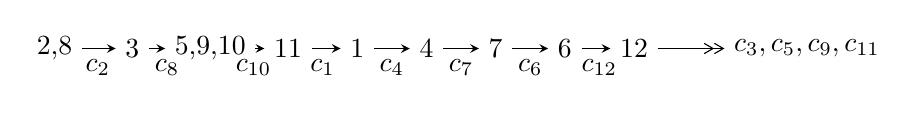
\begin{tikzpicture}[x=25pt, y=7pt]
	% node
	\node (A0) at (-1/8, 0) {2,8};
	\node (A1) at (1, 0) {3};
	\node (A2) at (17/8, 0) {5,9,10};
	\node (A3) at (13/4, 0) {11};
	\node (A4) at (17/4, 0) {1};
	\node (A5) at (21/4, 0) {4};
	\node (A6) at (25/4, 0) {7};
	\node (A7) at (29/4, 0) {6};
	\node (A8) at (33/4, 0) {12};
	\node (C1) at (1/2, -1) {$c_{2}$};
	\node (C2) at (3/2, -1) {$c_{8}$};
	\node (C3) at (11/4, -1) {$c_{10}$};
	\node (C4) at (15/4, -1) {$c_{1}$};
	\node (C5) at (19/4, -1) {$c_{4}$};
	\node (C6) at (23/4, -1) {$c_{7}$};
	\node (C7) at (27/4, -1) {$c_{6}$};
	\node (C8) at (31/4, -1) {$c_{12}$};
	\node (A9) at (43/4, 0) {$c_{3},c_{5},c_{9},c_{11}$};

	% edge
	\draw[->,>=stealth]	
	(A0) edge (A1) (A1) edge (A2) (A2) edge (A3) (A3) edge (A4) (A4) edge (A5) (A5) edge (A6) (A6) edge (A7) (A7) edge (A8) ;
	\draw[->>,>={angle 60}]	
	(A8) edge (A9);
\end{tikzpicture} \\ 

\end{tabular} \\

\footnotetext{
The image of knot diagram is generated by the software ``\textbf{Draw programme}" developed by Andrew Bartholomew(\url{http://www.layer8.co.uk/maths/draw/index.htm\#Running-draw}), where we modified some parts for our purpose(\url{https://github.com/CATsTAILs/LinksPainter}).
}\phantom \\ \newline 
\centering \textbf{Ideals for irreducible components\footnotemark of $X_{\text{par}}$} 
 
\begin{align*}
I^u_{1}&=\langle 
-23 u^{10}+17 u^9+u^8+31 u^7-65 u^6-55 u^5+74 u^4-34 u^3+84 u^2+356 d-316 u+56,\\
\phantom{I^u_{1}}&\phantom{= \langle  }-25 u^{10}+3 u^9-26 u^8-5 u^7-90 u^6-83 u^5-55 u^4-6 u^3-48 u^2+356 c-328 u-32,\\
\phantom{I^u_{1}}&\phantom{= \langle  }-21 u^{10}+31 u^9-61 u^8+67 u^7+49 u^6-27 u^5+114 u^4-240 u^3+216 u^2+356 b-304 u+144,\\
\phantom{I^u_{1}}&\phantom{= \langle  }4 u^{10}+28 u^9-35 u^8+72 u^7-39 u^6+56 u^5-9 u^4-234 u^3+86 u^2+356 a+24 u+176,\\
\phantom{I^u_{1}}&\phantom{= \langle  }u^{11}- u^{10}+2 u^9- u^8+2 u^7+3 u^6-3 u^5+4 u^4+12 u^2-4 u+4\rangle \\
I^u_{2}&=\langle 
- u^{16}-2 u^{14}-3 u^{12}-2 u^{10}- u^8+2 u^7-3 u^6+2 u^5-2 u^3+2 u^2+4 d-4 u,\\
\phantom{I^u_{2}}&\phantom{= \langle  }- u^{16}-3 u^{14}-6 u^{12}-7 u^{10}-6 u^8+2 u^7-6 u^6+4 u^5-4 u^4+4 u^3- u^2+4 c-2 u+2,\\
\phantom{I^u_{2}}&\phantom{= \langle  }u^{16}+2 u^{14}+5 u^{12}+6 u^{10}+7 u^8-2 u^7+7 u^6-2 u^5+2 u^4-6 u^3+4 u^2+4 b-4 u,\\
\phantom{I^u_{2}}&\phantom{= \langle  }-4 u^{16}+6 u^{15}+\cdots+4 a+6,\;u^{17}-2 u^{16}+\cdots-2 u+2\rangle \\
I^u_{3}&=\langle 
- u^{16}-2 u^{14}-3 u^{12}-2 u^{10}- u^8+2 u^7-3 u^6+2 u^5-2 u^3+2 u^2+4 d-4 u,\\
\phantom{I^u_{3}}&\phantom{= \langle  }- u^{16}-3 u^{14}-6 u^{12}-7 u^{10}-6 u^8+2 u^7-6 u^6+4 u^5-4 u^4+4 u^3- u^2+4 c-2 u+2,\\
\phantom{I^u_{3}}&\phantom{= \langle  }u^{16}-4 u^{15}+\cdots+4 b-4,\;2 u^{16}-4 u^{15}+\cdots+4 a-2,\;u^{17}-2 u^{16}+\cdots-2 u+2\rangle \\
I^u_{4}&=\langle 
2 u^{16}-4 u^{15}+\cdots+4 d-8,\;u^{11}+2 u^9+3 u^7- u^6+2 u^5- u^4+u^3-3 u^2+2 c+4 u-2,\\
\phantom{I^u_{4}}&\phantom{= \langle  }u^{16}-4 u^{15}+\cdots+4 b-4,\;2 u^{16}-4 u^{15}+\cdots+4 a-2,\;u^{17}-2 u^{16}+\cdots-2 u+2\rangle \\
I^u_{5}&=\langle 
- a^2 c- c a u- c a+d- c+a+u+1,\;a^2 c u+a^2 c+c a u+c^2- a u- a- u,\;a^2 u+a^2+a u+b- a,\\
\phantom{I^u_{5}}&\phantom{= \langle  }a^3+2 a^2 u+2 a^2+a u- u,\;u^2+u+1\rangle \\
\\
I^v_{1}&=\langle 
a,\;d,\;c+1,\;b-1,\;v+1\rangle \\
I^v_{2}&=\langle 
c,\;d+1,\;b,\;a-1,\;v+1\rangle \\
I^v_{3}&=\langle 
a,\;d+1,\;c+a,\;b-1,\;v+1\rangle \\
I^v_{4}&=\langle 
a,\;d a+c+1,\;d v-1,\;c v+a+v,\;b+1\rangle \\
\end{align*}
\raggedright * 8 irreducible components of $\dim_{\mathbb{C}}=0$, with total 77 representations.\\
\raggedright * 1 irreducible components of $\dim_{\mathbb{C}}=1$ \\
\footnotetext{All coefficients of polynomials are rational numbers. But the coefficients are sometimes approximated in decimal forms when there is not enough margin.}
\newpage
\renewcommand{\arraystretch}{1}
\centering \section*{I. $I^u_{1}= \langle -23 u^{10}+17 u^{9}+\cdots+356 d+56,\;-25 u^{10}+3 u^{9}+\cdots+356 c-32,\;-21 u^{10}+31 u^{9}+\cdots+356 b+144,\;4 u^{10}+28 u^9+\cdots+356 a+176,\;u^{11}- u^{10}+\cdots-4 u+4 \rangle$}
\flushleft \textbf{(i) Arc colorings}\\
\begin{tabular}{m{7pt} m{180pt} m{7pt} m{180pt} }
\flushright $a_{2}=$&$\begin{pmatrix}1\\0\end{pmatrix}$ \\
\flushright $a_{8}=$&$\begin{pmatrix}0\\u\end{pmatrix}$ \\
\flushright $a_{3}=$&$\begin{pmatrix}1\\- u^2\end{pmatrix}$ \\
\flushright $a_{5}=$&$\begin{pmatrix}-0.0112360 u^{10}-0.0786517 u^{9}+\cdots-0.0674157 u-0.494382\\0.0589888 u^{10}-0.0870787 u^{9}+\cdots+0.853933 u-0.404494\end{pmatrix}$ \\
\flushright $a_{9}=$&$\begin{pmatrix}u\\u\end{pmatrix}$ \\
\flushright $a_{10}=$&$\begin{pmatrix}0.0702247 u^{10}-0.00842697 u^{9}+\cdots+0.921348 u+0.0898876\\0.0646067 u^{10}-0.0477528 u^{9}+\cdots+0.887640 u-0.157303\end{pmatrix}$ \\
\flushright $a_{11}=$&$\begin{pmatrix}0.140449 u^{10}-0.0168539 u^{9}+\cdots+0.842697 u+0.179775\\0.134831 u^{10}-0.0561798 u^{9}+\cdots+0.808989 u-0.0674157\end{pmatrix}$ \\
\flushright $a_{1}=$&$\begin{pmatrix}u^2+1\\- u^4\end{pmatrix}$ \\
\flushright $a_{4}=$&$\begin{pmatrix}0.00561798 u^{10}+0.0393258 u^{9}+\cdots+0.0337079 u-0.752809\\-0.0646067 u^{10}+0.0477528 u^{9}+\cdots+0.112360 u+0.157303\end{pmatrix}$ \\
\flushright $a_{7}=$&$\begin{pmatrix}-0.00561798 u^{10}-0.0393258 u^{9}+\cdots-0.0337079 u-0.247191\\0.0646067 u^{10}-0.0477528 u^{9}+\cdots+0.887640 u-0.157303\end{pmatrix}$ \\
\flushright $a_{6}=$&$\begin{pmatrix}-0.0112360 u^{10}-0.0786517 u^{9}+\cdots-0.0674157 u-0.494382\\0.0589888 u^{10}-0.0870787 u^{9}+\cdots+0.853933 u-0.404494\end{pmatrix}$ \\
\flushright $a_{12}=$&$\begin{pmatrix}0.101124 u^{10}-0.0421348 u^{9}+\cdots+0.606742 u+0.449438\\0.0898876 u^{10}-0.120787 u^{9}+\cdots+0.539326 u-0.0449438\end{pmatrix}$\\&\end{tabular}
\flushleft \textbf{(ii) Obstruction class $= -1$}\\~\\
\flushleft \textbf{(iii) Cusp Shapes $= -\frac{113}{89} u^{10}+\frac{99}{89} u^9-\frac{146}{89} u^8+\frac{13}{89} u^7-\frac{122}{89} u^6-\frac{247}{89} u^5+\frac{321}{89} u^4-\frac{20}{89} u^3-\frac{338}{89} u^2-\frac{1212}{89} u-\frac{522}{89}$}\\~\\
\newpage\renewcommand{\arraystretch}{1}
\flushleft \textbf{(iv) u-Polynomials at the component}\newline \\
\begin{tabular}{m{50pt}|m{274pt}}
Crossings & \hspace{64pt}u-Polynomials at each crossing \\
\hline $$\begin{aligned}c_{1}\end{aligned}$$&$\begin{aligned}
&u^{11}+3 u^{10}+\cdots-80 u-16
\end{aligned}$\\
\hline $$\begin{aligned}c_{2},c_{8}\end{aligned}$$&$\begin{aligned}
&u^{11}- u^{10}+2 u^9- u^8+2 u^7+3 u^6-3 u^5+4 u^4+12 u^2-4 u+4
\end{aligned}$\\
\hline $$\begin{aligned}c_{3},c_{4},c_{5}\\c_{6},c_{7},c_{9}\\c_{10},c_{11},c_{12}\end{aligned}$$&$\begin{aligned}
&u^{11}- u^{10}-6 u^9+5 u^8+13 u^7-7 u^6-10 u^5-2 u^4-2 u^3+8 u^2+4 u+1
\end{aligned}$\\
\hline
\end{tabular}\\~\\
\newpage\renewcommand{\arraystretch}{1}
\flushleft \textbf{(v) Riley Polynomials at the component}\newline \\
\begin{tabular}{m{50pt}|m{274pt}}
Crossings & \hspace{64pt}Riley Polynomials at each crossing \\
\hline $$\begin{aligned}c_{1}\end{aligned}$$&$\begin{aligned}
&y^{11}+3 y^{10}+\cdots+768 y-256
\end{aligned}$\\
\hline $$\begin{aligned}c_{2},c_{8}\end{aligned}$$&$\begin{aligned}
&y^{11}+3 y^{10}+\cdots-80 y-16
\end{aligned}$\\
\hline $$\begin{aligned}c_{3},c_{4},c_{5}\\c_{6},c_{7},c_{9}\\c_{10},c_{11},c_{12}\end{aligned}$$&$\begin{aligned}
&y^{11}-13 y^{10}+\cdots-76 y^2-1
\end{aligned}$\\
\hline
\end{tabular}\\~\\
\newpage\flushleft \textbf{(vi) Complex Volumes and Cusp Shapes}
$$\begin{array}{c|c|c}  
\text{Solutions to }I^u_{1}& \I (\text{vol} + \sqrt{-1}CS) & \text{Cusp shape}\\
 \hline 
\begin{aligned}
u &= -0.697658 + 0.849048 I \\
a &= \phantom{-}0.921136 + 0.783422 I \\
b &= \phantom{-}0.740581 + 0.864357 I \\
c &= -0.485430 + 0.499909 I \\
d &= -0.063398 + 0.826398 I\end{aligned}
 & \phantom{-}3.70211 - 2.67058 I & -3.05924 + 3.87935 I \\ \hline\begin{aligned}
u &= -0.697658 - 0.849048 I \\
a &= \phantom{-}0.921136 - 0.783422 I \\
b &= \phantom{-}0.740581 - 0.864357 I \\
c &= -0.485430 - 0.499909 I \\
d &= -0.063398 - 0.826398 I\end{aligned}
 & \phantom{-}3.70211 + 2.67058 I & -3.05924 - 3.87935 I \\ \hline\begin{aligned}
u &= -1.27716\phantom{ +0.000000I} \\
a &= \phantom{-}1.30381\phantom{ +0.000000I} \\
b &= -1.87182\phantom{ +0.000000I} \\
c &= \phantom{-}1.14011\phantom{ +0.000000I} \\
d &= -0.519995\phantom{ +0.000000I}\end{aligned}
 & -13.3802\phantom{ +0.000000I} & -18.2600\phantom{ +0.000000I} \\ \hline\begin{aligned}
u &= \phantom{-}1.147220 + 0.649373 I \\
a &= -0.08285 + 1.84843 I \\
b &= \phantom{-}1.76297 - 0.05107 I \\
c &= -1.037550 + 0.312280 I \\
d &= \phantom{-}0.506365 + 0.204596 I\end{aligned}
 & -9.05799 - 8.57514 I & -15.6343 + 5.1528 I \\ \hline\begin{aligned}
u &= \phantom{-}1.147220 - 0.649373 I \\
a &= -0.08285 - 1.84843 I \\
b &= \phantom{-}1.76297 + 0.05107 I \\
c &= -1.037550 - 0.312280 I \\
d &= \phantom{-}0.506365 - 0.204596 I\end{aligned}
 & -9.05799 + 8.57514 I & -15.6343 - 5.1528 I \\ \hline\begin{aligned}
u &= \phantom{-}0.188962 + 0.548520 I \\
a &= -0.556629 - 0.158029 I \\
b &= -0.197361 + 0.297672 I \\
c &= \phantom{-}0.248124 + 0.521791 I \\
d &= \phantom{-}0.066277 + 0.455147 I\end{aligned}
 & -0.301659 + 0.791298 I & -7.48686 - 8.65650 I\\
 \hline 
 \end{array}$$\newpage$$\begin{array}{c|c|c}  
\text{Solutions to }I^u_{1}& \I (\text{vol} + \sqrt{-1}CS) & \text{Cusp shape}\\
 \hline 
\begin{aligned}
u &= \phantom{-}0.188962 - 0.548520 I \\
a &= -0.556629 + 0.158029 I \\
b &= -0.197361 - 0.297672 I \\
c &= \phantom{-}0.248124 - 0.521791 I \\
d &= \phantom{-}0.066277 - 0.455147 I\end{aligned}
 & -0.301659 - 0.791298 I & -7.48686 + 8.65650 I \\ \hline\begin{aligned}
u &= \phantom{-}0.80937 + 1.18781 I \\
a &= -1.69324 - 0.30290 I \\
b &= -3.40094 + 1.12656 I \\
c &= \phantom{-}0.326968 - 0.969070 I \\
d &= \phantom{-}0.40614 - 2.47046 I\end{aligned}
 & -10.8529 + 15.6015 I & -15.8571 - 8.6135 I \\ \hline\begin{aligned}
u &= \phantom{-}0.80937 - 1.18781 I \\
a &= -1.69324 + 0.30290 I \\
b &= -3.40094 - 1.12656 I \\
c &= \phantom{-}0.326968 + 0.969070 I \\
d &= \phantom{-}0.40614 + 2.47046 I\end{aligned}
 & -10.8529 - 15.6015 I & -15.8571 + 8.6135 I \\ \hline\begin{aligned}
u &= -0.30932 + 1.43197 I \\
a &= \phantom{-}0.759680 + 0.558726 I \\
b &= \phantom{-}1.53066 + 2.95790 I \\
c &= -0.122169 - 1.042440 I \\
d &= -0.15539 - 2.65594 I\end{aligned}
 & -18.7453 - 5.8080 I & -19.8325 + 3.5503 I \\ \hline\begin{aligned}
u &= -0.30932 - 1.43197 I \\
a &= \phantom{-}0.759680 - 0.558726 I \\
b &= \phantom{-}1.53066 - 2.95790 I \\
c &= -0.122169 + 1.042440 I \\
d &= -0.15539 + 2.65594 I\end{aligned}
 & -18.7453 + 5.8080 I & -19.8325 - 3.5503 I\\
 \hline 
 \end{array}$$\newpage\newpage\renewcommand{\arraystretch}{1}
\centering \section*{II. $I^u_{2}= \langle - u^{16}-2 u^{14}+\cdots+4 d-4 u,\;- u^{16}-3 u^{14}+\cdots+4 c+2,\;u^{16}+2 u^{14}+\cdots+4 b-4 u,\;-4 u^{16}+6 u^{15}+\cdots+4 a+6,\;u^{17}-2 u^{16}+\cdots-2 u+2 \rangle$}
\flushleft \textbf{(i) Arc colorings}\\
\begin{tabular}{m{7pt} m{180pt} m{7pt} m{180pt} }
\flushright $a_{2}=$&$\begin{pmatrix}1\\0\end{pmatrix}$ \\
\flushright $a_{8}=$&$\begin{pmatrix}0\\u\end{pmatrix}$ \\
\flushright $a_{3}=$&$\begin{pmatrix}1\\- u^2\end{pmatrix}$ \\
\flushright $a_{5}=$&$\begin{pmatrix}u^{16}-\frac{3}{2} u^{15}+\cdots+2 u-\frac{3}{2}\\-\frac{1}{4} u^{16}-\frac{1}{2} u^{14}+\cdots- u^2+u\end{pmatrix}$ \\
\flushright $a_{9}=$&$\begin{pmatrix}u\\u\end{pmatrix}$ \\
\flushright $a_{10}=$&$\begin{pmatrix}\frac{1}{4} u^{16}+\frac{3}{4} u^{14}+\cdots+\frac{1}{2} u-\frac{1}{2}\\\frac{1}{4} u^{16}+\frac{1}{2} u^{14}+\cdots-\frac{1}{2} u^2+u\end{pmatrix}$ \\
\flushright $a_{11}=$&$\begin{pmatrix}- u^{16}+\frac{3}{2} u^{15}+\cdots-\frac{3}{2} u+1\\\frac{1}{2} u^{14}+u^{12}+\cdots- u^3-1\end{pmatrix}$ \\
\flushright $a_{1}=$&$\begin{pmatrix}u^2+1\\- u^4\end{pmatrix}$ \\
\flushright $a_{4}=$&$\begin{pmatrix}u^{16}-\frac{3}{2} u^{15}+\cdots+3 u-\frac{3}{2}\\\frac{1}{4} u^{16}+\frac{1}{2} u^{14}+\cdots- u^2+u\end{pmatrix}$ \\
\flushright $a_{7}=$&$\begin{pmatrix}-\frac{1}{4} u^{14}-\frac{3}{4} u^{12}+\cdots+\frac{1}{2} u+\frac{1}{2}\\\frac{1}{4} u^{16}+\frac{1}{2} u^{14}+\cdots-\frac{1}{2} u^2+u\end{pmatrix}$ \\
\flushright $a_{6}=$&$\begin{pmatrix}\frac{1}{2} u^{16}- u^{15}+\cdots+u-\frac{1}{2}\\\frac{3}{4} u^{16}- u^{15}+\cdots+\frac{3}{2} u-1\end{pmatrix}$ \\
\flushright $a_{12}=$&$\begin{pmatrix}- u^{16}+\frac{3}{2} u^{15}+\cdots-2 u+\frac{1}{2}\\\frac{1}{4} u^{14}+\frac{1}{2} u^{12}+\cdots+\frac{3}{4} u^4-1\end{pmatrix}$\\&\end{tabular}
\flushleft \textbf{(ii) Obstruction class $= -1$}\\~\\
\flushleft \textbf{(iii) Cusp Shapes $= -2 u^{16}+4 u^{15}-6 u^{14}+8 u^{13}-8 u^{12}+14 u^{11}-10 u^{10}+12 u^9-4 u^8+10 u^7-20 u^6+26 u^5-16 u^4-4 u^3+10 u^2-8 u-8$}\\~\\
\newpage\renewcommand{\arraystretch}{1}
\flushleft \textbf{(iv) u-Polynomials at the component}\newline \\
\begin{tabular}{m{50pt}|m{274pt}}
Crossings & \hspace{64pt}u-Polynomials at each crossing \\
\hline $$\begin{aligned}c_{1}\end{aligned}$$&$\begin{aligned}
&u^{17}+6 u^{16}+\cdots+8 u-4
\end{aligned}$\\
\hline $$\begin{aligned}c_{2},c_{8}\end{aligned}$$&$\begin{aligned}
&u^{17}-2 u^{16}+\cdots-2 u+2
\end{aligned}$\\
\hline $$\begin{aligned}c_{3},c_{4},c_{12}\end{aligned}$$&$\begin{aligned}
&u^{17}-5 u^{15}+\cdots-3 u^2+4
\end{aligned}$\\
\hline $$\begin{aligned}c_{5},c_{6},c_{7}\\c_{9},c_{10},c_{11}\end{aligned}$$&$\begin{aligned}
&u^{17}-2 u^{16}+\cdots+3 u-1
\end{aligned}$\\
\hline
\end{tabular}\\~\\
\newpage\renewcommand{\arraystretch}{1}
\flushleft \textbf{(v) Riley Polynomials at the component}\newline \\
\begin{tabular}{m{50pt}|m{274pt}}
Crossings & \hspace{64pt}Riley Polynomials at each crossing \\
\hline $$\begin{aligned}c_{1}\end{aligned}$$&$\begin{aligned}
&y^{17}+6 y^{16}+\cdots+376 y-16
\end{aligned}$\\
\hline $$\begin{aligned}c_{2},c_{8}\end{aligned}$$&$\begin{aligned}
&y^{17}+6 y^{16}+\cdots+8 y-4
\end{aligned}$\\
\hline $$\begin{aligned}c_{3},c_{4},c_{12}\end{aligned}$$&$\begin{aligned}
&y^{17}-10 y^{16}+\cdots+24 y-16
\end{aligned}$\\
\hline $$\begin{aligned}c_{5},c_{6},c_{7}\\c_{9},c_{10},c_{11}\end{aligned}$$&$\begin{aligned}
&y^{17}-16 y^{16}+\cdots+19 y-1
\end{aligned}$\\
\hline
\end{tabular}\\~\\
\newpage\flushleft \textbf{(vi) Complex Volumes and Cusp Shapes}
$$\begin{array}{c|c|c}  
\text{Solutions to }I^u_{2}& \I (\text{vol} + \sqrt{-1}CS) & \text{Cusp shape}\\
 \hline 
\begin{aligned}
u &= \phantom{-}0.742615 + 0.650908 I \\
a &= -0.718435 + 0.821804 I \\
b &= -0.566230 + 1.035510 I \\
c &= \phantom{-}0.489237 + 0.474516 I \\
d &= \phantom{-}0.197556 + 0.828548 I\end{aligned}
 & \phantom{-}0.369365 - 1.227240 I & -5.85153 + 0.85505 I \\ \hline\begin{aligned}
u &= \phantom{-}0.742615 - 0.650908 I \\
a &= -0.718435 - 0.821804 I \\
b &= -0.566230 - 1.035510 I \\
c &= \phantom{-}0.489237 - 0.474516 I \\
d &= \phantom{-}0.197556 - 0.828548 I\end{aligned}
 & \phantom{-}0.369365 + 1.227240 I & -5.85153 - 0.85505 I \\ \hline\begin{aligned}
u &= \phantom{-}0.834865 + 0.265014 I \\
a &= -2.92918 + 3.22304 I \\
b &= \phantom{-}1.94336 - 0.16531 I \\
c &= -1.39610 + 0.29715 I \\
d &= \phantom{-}0.377294 + 0.097590 I\end{aligned}
 & -5.90943 - 0.43387 I & -14.5683 - 0.8754 I \\ \hline\begin{aligned}
u &= \phantom{-}0.834865 - 0.265014 I \\
a &= -2.92918 - 3.22304 I \\
b &= \phantom{-}1.94336 + 0.16531 I \\
c &= -1.39610 - 0.29715 I \\
d &= \phantom{-}0.377294 - 0.097590 I\end{aligned}
 & -5.90943 + 0.43387 I & -14.5683 + 0.8754 I \\ \hline\begin{aligned}
u &= -0.976738 + 0.562668 I \\
a &= \phantom{-}0.35073 + 2.53095 I \\
b &= -1.77103 - 0.11938 I \\
c &= \phantom{-}1.124900 + 0.370279 I \\
d &= -0.445879 + 0.191459 I\end{aligned}
 & -3.90030 + 4.64771 I & -11.56085 - 4.11695 I \\ \hline\begin{aligned}
u &= -0.976738 - 0.562668 I \\
a &= \phantom{-}0.35073 - 2.53095 I \\
b &= -1.77103 + 0.11938 I \\
c &= \phantom{-}1.124900 - 0.370279 I \\
d &= -0.445879 - 0.191459 I\end{aligned}
 & -3.90030 - 4.64771 I & -11.56085 + 4.11695 I\\
 \hline 
 \end{array}$$\newpage$$\begin{array}{c|c|c}  
\text{Solutions to }I^u_{2}& \I (\text{vol} + \sqrt{-1}CS) & \text{Cusp shape}\\
 \hline 
\begin{aligned}
u &= \phantom{-}0.003992 + 0.842342 I \\
a &= \phantom{-}2.04176 + 0.02534 I \\
b &= \phantom{-}0.770137 - 0.000913 I \\
c &= -0.499289 + 0.745483 I \\
d &= \phantom{-}0.126546 + 0.484371 I\end{aligned}
 & -4.59969 - 1.46955 I & -15.6358 + 4.6653 I \\ \hline\begin{aligned}
u &= \phantom{-}0.003992 - 0.842342 I \\
a &= \phantom{-}2.04176 - 0.02534 I \\
b &= \phantom{-}0.770137 + 0.000913 I \\
c &= -0.499289 - 0.745483 I \\
d &= \phantom{-}0.126546 - 0.484371 I\end{aligned}
 & -4.59969 + 1.46955 I & -15.6358 - 4.6653 I \\ \hline\begin{aligned}
u &= \phantom{-}0.656745 + 1.004700 I \\
a &= -1.055980 + 0.795426 I \\
b &= -0.860931 + 0.769831 I \\
c &= \phantom{-}0.494032 + 0.511989 I \\
d &= -0.026089 + 0.826073 I\end{aligned}
 & -0.71009 + 6.57063 I & -8.73995 - 6.43452 I \\ \hline\begin{aligned}
u &= \phantom{-}0.656745 - 1.004700 I \\
a &= -1.055980 - 0.795426 I \\
b &= -0.860931 - 0.769831 I \\
c &= \phantom{-}0.494032 - 0.511989 I \\
d &= -0.026089 - 0.826073 I\end{aligned}
 & -0.71009 - 6.57063 I & -8.73995 + 6.43452 I \\ \hline\begin{aligned}
u &= \phantom{-}0.110097 + 1.246510 I \\
a &= -0.44777 + 1.36378 I \\
b &= -0.91154 + 4.59961 I \\
c &= \phantom{-}0.059575 - 1.151130 I \\
d &= \phantom{-}0.08505 - 2.81355 I\end{aligned}
 & -11.32450 + 2.71165 I & -17.8424 - 3.1371 I \\ \hline\begin{aligned}
u &= \phantom{-}0.110097 - 1.246510 I \\
a &= -0.44777 - 1.36378 I \\
b &= -0.91154 - 4.59961 I \\
c &= \phantom{-}0.059575 + 1.151130 I \\
d &= \phantom{-}0.08505 + 2.81355 I\end{aligned}
 & -11.32450 - 2.71165 I & -17.8424 + 3.1371 I\\
 \hline 
 \end{array}$$\newpage$$\begin{array}{c|c|c}  
\text{Solutions to }I^u_{2}& \I (\text{vol} + \sqrt{-1}CS) & \text{Cusp shape}\\
 \hline 
\begin{aligned}
u &= \phantom{-}0.578864 + 1.116300 I \\
a &= -1.94591 + 0.31220 I \\
b &= -3.95970 + 2.40372 I \\
c &= \phantom{-}0.306410 - 1.074930 I \\
d &= \phantom{-}0.42725 - 2.64129 I\end{aligned}
 & -8.33968 + 5.51158 I & -16.2513 - 3.8449 I \\ \hline\begin{aligned}
u &= \phantom{-}0.578864 - 1.116300 I \\
a &= -1.94591 - 0.31220 I \\
b &= -3.95970 - 2.40372 I \\
c &= \phantom{-}0.306410 + 1.074930 I \\
d &= \phantom{-}0.42725 + 2.64129 I\end{aligned}
 & -8.33968 - 5.51158 I & -16.2513 + 3.8449 I \\ \hline\begin{aligned}
u &= -0.718492 + 1.129370 I \\
a &= \phantom{-}1.87724 - 0.11825 I \\
b &= \phantom{-}3.79947 + 1.50560 I \\
c &= -0.334233 - 1.013370 I \\
d &= -0.44170 - 2.53369 I\end{aligned}
 & -5.69311 - 10.83370 I & -12.8938 + 7.4126 I \\ \hline\begin{aligned}
u &= -0.718492 - 1.129370 I \\
a &= \phantom{-}1.87724 + 0.11825 I \\
b &= \phantom{-}3.79947 - 1.50560 I \\
c &= -0.334233 + 1.013370 I \\
d &= -0.44170 + 2.53369 I\end{aligned}
 & -5.69311 + 10.83370 I & -12.8938 - 7.4126 I \\ \hline\begin{aligned}
u &= -0.463897\phantom{ +0.000000I} \\
a &= -0.344922\phantom{ +0.000000I} \\
b &= -0.887074\phantom{ +0.000000I} \\
c &= -0.489071\phantom{ +0.000000I} \\
d &= -0.600031\phantom{ +0.000000I}\end{aligned}
 & -2.03175\phantom{ +0.000000I} & -3.31210\phantom{ +0.000000I}\\
 \hline 
 \end{array}$$\newpage\newpage\renewcommand{\arraystretch}{1}
\centering \section*{III. $I^u_{3}= \langle - u^{16}-2 u^{14}+\cdots+4 d-4 u,\;- u^{16}-3 u^{14}+\cdots+4 c+2,\;u^{16}-4 u^{15}+\cdots+4 b-4,\;2 u^{16}-4 u^{15}+\cdots+4 a-2,\;u^{17}-2 u^{16}+\cdots-2 u+2 \rangle$}
\flushleft \textbf{(i) Arc colorings}\\
\begin{tabular}{m{7pt} m{180pt} m{7pt} m{180pt} }
\flushright $a_{2}=$&$\begin{pmatrix}1\\0\end{pmatrix}$ \\
\flushright $a_{8}=$&$\begin{pmatrix}0\\u\end{pmatrix}$ \\
\flushright $a_{3}=$&$\begin{pmatrix}1\\- u^2\end{pmatrix}$ \\
\flushright $a_{5}=$&$\begin{pmatrix}-\frac{1}{2} u^{16}+u^{15}+\cdots-\frac{11}{4} u^2+\frac{1}{2}\\-\frac{1}{4} u^{16}+u^{15}+\cdots-\frac{3}{2} u+1\end{pmatrix}$ \\
\flushright $a_{9}=$&$\begin{pmatrix}u\\u\end{pmatrix}$ \\
\flushright $a_{10}=$&$\begin{pmatrix}\frac{1}{4} u^{16}+\frac{3}{4} u^{14}+\cdots+\frac{1}{2} u-\frac{1}{2}\\\frac{1}{4} u^{16}+\frac{1}{2} u^{14}+\cdots-\frac{1}{2} u^2+u\end{pmatrix}$ \\
\flushright $a_{11}=$&$\begin{pmatrix}\frac{1}{2} u^{16}+\frac{3}{2} u^{14}+\cdots+\frac{5}{2} u^2-\frac{1}{2} u\\u^{15}- u^{14}+\cdots-2 u^2+1\end{pmatrix}$ \\
\flushright $a_{1}=$&$\begin{pmatrix}u^2+1\\- u^4\end{pmatrix}$ \\
\flushright $a_{4}=$&$\begin{pmatrix}\frac{1}{4} u^{13}+\frac{1}{2} u^{11}+\cdots- u^2-1\\\frac{1}{4} u^{13}+\frac{1}{2} u^{11}+\cdots+\frac{1}{2} u^2-\frac{1}{2} u\end{pmatrix}$ \\
\flushright $a_{7}=$&$\begin{pmatrix}-\frac{1}{4} u^{14}-\frac{3}{4} u^{12}+\cdots+\frac{1}{2} u+\frac{1}{2}\\\frac{1}{4} u^{16}+\frac{1}{2} u^{14}+\cdots-\frac{1}{2} u^2+u\end{pmatrix}$ \\
\flushright $a_{6}=$&$\begin{pmatrix}\frac{1}{2} u^{16}- u^{15}+\cdots+u-\frac{1}{2}\\\frac{3}{4} u^{16}- u^{15}+\cdots+\frac{3}{2} u-1\end{pmatrix}$ \\
\flushright $a_{12}=$&$\begin{pmatrix}\frac{1}{2} u^{16}-\frac{1}{4} u^{15}+\cdots-\frac{1}{2} u+\frac{1}{2}\\\frac{3}{4} u^{15}-\frac{3}{4} u^{14}+\cdots-\frac{1}{2} u+1\end{pmatrix}$\\&\end{tabular}
\flushleft \textbf{(ii) Obstruction class $= -1$}\\~\\
\flushleft \textbf{(iii) Cusp Shapes $= -2 u^{16}+4 u^{15}-6 u^{14}+8 u^{13}-8 u^{12}+14 u^{11}-10 u^{10}+12 u^9-4 u^8+10 u^7-20 u^6+26 u^5-16 u^4-4 u^3+10 u^2-8 u-8$}\\~\\
\newpage\renewcommand{\arraystretch}{1}
\flushleft \textbf{(iv) u-Polynomials at the component}\newline \\
\begin{tabular}{m{50pt}|m{274pt}}
Crossings & \hspace{64pt}u-Polynomials at each crossing \\
\hline $$\begin{aligned}c_{1}\end{aligned}$$&$\begin{aligned}
&u^{17}+6 u^{16}+\cdots+8 u-4
\end{aligned}$\\
\hline $$\begin{aligned}c_{2},c_{8}\end{aligned}$$&$\begin{aligned}
&u^{17}-2 u^{16}+\cdots-2 u+2
\end{aligned}$\\
\hline $$\begin{aligned}c_{3},c_{4},c_{6}\\c_{7},c_{9},c_{12}\end{aligned}$$&$\begin{aligned}
&u^{17}-2 u^{16}+\cdots+3 u-1
\end{aligned}$\\
\hline $$\begin{aligned}c_{5},c_{10},c_{11}\end{aligned}$$&$\begin{aligned}
&u^{17}-5 u^{15}+\cdots-3 u^2+4
\end{aligned}$\\
\hline
\end{tabular}\\~\\
\newpage\renewcommand{\arraystretch}{1}
\flushleft \textbf{(v) Riley Polynomials at the component}\newline \\
\begin{tabular}{m{50pt}|m{274pt}}
Crossings & \hspace{64pt}Riley Polynomials at each crossing \\
\hline $$\begin{aligned}c_{1}\end{aligned}$$&$\begin{aligned}
&y^{17}+6 y^{16}+\cdots+376 y-16
\end{aligned}$\\
\hline $$\begin{aligned}c_{2},c_{8}\end{aligned}$$&$\begin{aligned}
&y^{17}+6 y^{16}+\cdots+8 y-4
\end{aligned}$\\
\hline $$\begin{aligned}c_{3},c_{4},c_{6}\\c_{7},c_{9},c_{12}\end{aligned}$$&$\begin{aligned}
&y^{17}-16 y^{16}+\cdots+19 y-1
\end{aligned}$\\
\hline $$\begin{aligned}c_{5},c_{10},c_{11}\end{aligned}$$&$\begin{aligned}
&y^{17}-10 y^{16}+\cdots+24 y-16
\end{aligned}$\\
\hline
\end{tabular}\\~\\
\newpage\flushleft \textbf{(vi) Complex Volumes and Cusp Shapes}
$$\begin{array}{c|c|c}  
\text{Solutions to }I^u_{3}& \I (\text{vol} + \sqrt{-1}CS) & \text{Cusp shape}\\
 \hline 
\begin{aligned}
u &= \phantom{-}0.742615 + 0.650908 I \\
a &= \phantom{-}0.33067 - 1.38135 I \\
b &= -0.289061 - 0.354565 I \\
c &= \phantom{-}0.489237 + 0.474516 I \\
d &= \phantom{-}0.197556 + 0.828548 I\end{aligned}
 & \phantom{-}0.369365 - 1.227240 I & -5.85153 + 0.85505 I \\ \hline\begin{aligned}
u &= \phantom{-}0.742615 - 0.650908 I \\
a &= \phantom{-}0.33067 + 1.38135 I \\
b &= -0.289061 + 0.354565 I \\
c &= \phantom{-}0.489237 - 0.474516 I \\
d &= \phantom{-}0.197556 - 0.828548 I\end{aligned}
 & \phantom{-}0.369365 + 1.227240 I & -5.85153 - 0.85505 I \\ \hline\begin{aligned}
u &= \phantom{-}0.834865 + 0.265014 I \\
a &= -0.007441 + 0.469677 I \\
b &= -0.594985 + 0.032560 I \\
c &= -1.39610 + 0.29715 I \\
d &= \phantom{-}0.377294 + 0.097590 I\end{aligned}
 & -5.90943 - 0.43387 I & -14.5683 - 0.8754 I \\ \hline\begin{aligned}
u &= \phantom{-}0.834865 - 0.265014 I \\
a &= -0.007441 - 0.469677 I \\
b &= -0.594985 - 0.032560 I \\
c &= -1.39610 - 0.29715 I \\
d &= \phantom{-}0.377294 - 0.097590 I\end{aligned}
 & -5.90943 + 0.43387 I & -14.5683 + 0.8754 I \\ \hline\begin{aligned}
u &= -0.976738 + 0.562668 I \\
a &= -0.220338 - 1.221990 I \\
b &= \phantom{-}0.383732 - 0.363700 I \\
c &= \phantom{-}1.124900 + 0.370279 I \\
d &= -0.445879 + 0.191459 I\end{aligned}
 & -3.90030 + 4.64771 I & -11.56085 - 4.11695 I \\ \hline\begin{aligned}
u &= -0.976738 - 0.562668 I \\
a &= -0.220338 + 1.221990 I \\
b &= \phantom{-}0.383732 + 0.363700 I \\
c &= \phantom{-}1.124900 - 0.370279 I \\
d &= -0.445879 - 0.191459 I\end{aligned}
 & -3.90030 - 4.64771 I & -11.56085 + 4.11695 I\\
 \hline 
 \end{array}$$\newpage$$\begin{array}{c|c|c}  
\text{Solutions to }I^u_{3}& \I (\text{vol} + \sqrt{-1}CS) & \text{Cusp shape}\\
 \hline 
\begin{aligned}
u &= \phantom{-}0.003992 + 0.842342 I \\
a &= -0.617996 - 0.253084 I \\
b &= -1.11240 - 0.99360 I \\
c &= -0.499289 + 0.745483 I \\
d &= \phantom{-}0.126546 + 0.484371 I\end{aligned}
 & -4.59969 - 1.46955 I & -15.6358 + 4.6653 I \\ \hline\begin{aligned}
u &= \phantom{-}0.003992 - 0.842342 I \\
a &= -0.617996 + 0.253084 I \\
b &= -1.11240 + 0.99360 I \\
c &= -0.499289 - 0.745483 I \\
d &= \phantom{-}0.126546 - 0.484371 I\end{aligned}
 & -4.59969 + 1.46955 I & -15.6358 - 4.6653 I \\ \hline\begin{aligned}
u &= \phantom{-}0.656745 + 1.004700 I \\
a &= \phantom{-}1.271870 - 0.179063 I \\
b &= \phantom{-}2.14507 - 0.73367 I \\
c &= \phantom{-}0.494032 + 0.511989 I \\
d &= -0.026089 + 0.826073 I\end{aligned}
 & -0.71009 + 6.57063 I & -8.73995 - 6.43452 I \\ \hline\begin{aligned}
u &= \phantom{-}0.656745 - 1.004700 I \\
a &= \phantom{-}1.271870 + 0.179063 I \\
b &= \phantom{-}2.14507 + 0.73367 I \\
c &= \phantom{-}0.494032 - 0.511989 I \\
d &= -0.026089 - 0.826073 I\end{aligned}
 & -0.71009 - 6.57063 I & -8.73995 + 6.43452 I \\ \hline\begin{aligned}
u &= \phantom{-}0.110097 + 1.246510 I \\
a &= \phantom{-}0.925043 - 0.007268 I \\
b &= \phantom{-}1.55691 - 0.59036 I \\
c &= \phantom{-}0.059575 - 1.151130 I \\
d &= \phantom{-}0.08505 - 2.81355 I\end{aligned}
 & -11.32450 + 2.71165 I & -17.8424 - 3.1371 I \\ \hline\begin{aligned}
u &= \phantom{-}0.110097 - 1.246510 I \\
a &= \phantom{-}0.925043 + 0.007268 I \\
b &= \phantom{-}1.55691 + 0.59036 I \\
c &= \phantom{-}0.059575 + 1.151130 I \\
d &= \phantom{-}0.08505 + 2.81355 I\end{aligned}
 & -11.32450 - 2.71165 I & -17.8424 + 3.1371 I\\
 \hline 
 \end{array}$$\newpage$$\begin{array}{c|c|c}  
\text{Solutions to }I^u_{3}& \I (\text{vol} + \sqrt{-1}CS) & \text{Cusp shape}\\
 \hline 
\begin{aligned}
u &= \phantom{-}0.578864 + 1.116300 I \\
a &= -0.594829 + 0.285325 I \\
b &= -1.098970 - 0.234758 I \\
c &= \phantom{-}0.306410 - 1.074930 I \\
d &= \phantom{-}0.42725 - 2.64129 I\end{aligned}
 & -8.33968 + 5.51158 I & -16.2513 - 3.8449 I \\ \hline\begin{aligned}
u &= \phantom{-}0.578864 - 1.116300 I \\
a &= -0.594829 - 0.285325 I \\
b &= -1.098970 + 0.234758 I \\
c &= \phantom{-}0.306410 + 1.074930 I \\
d &= \phantom{-}0.42725 + 2.64129 I\end{aligned}
 & -8.33968 - 5.51158 I & -16.2513 + 3.8449 I \\ \hline\begin{aligned}
u &= -0.718492 + 1.129370 I \\
a &= -1.276660 - 0.102756 I \\
b &= -2.11452 - 0.60757 I \\
c &= -0.334233 - 1.013370 I \\
d &= -0.44170 - 2.53369 I\end{aligned}
 & -5.69311 - 10.83370 I & -12.8938 + 7.4126 I \\ \hline\begin{aligned}
u &= -0.718492 - 1.129370 I \\
a &= -1.276660 + 0.102756 I \\
b &= -2.11452 + 0.60757 I \\
c &= -0.334233 + 1.013370 I \\
d &= -0.44170 + 2.53369 I\end{aligned}
 & -5.69311 + 10.83370 I & -12.8938 - 7.4126 I \\ \hline\begin{aligned}
u &= -0.463897\phantom{ +0.000000I} \\
a &= -1.62063\phantom{ +0.000000I} \\
b &= \phantom{-}0.248463\phantom{ +0.000000I} \\
c &= -0.489071\phantom{ +0.000000I} \\
d &= -0.600031\phantom{ +0.000000I}\end{aligned}
 & -2.03175\phantom{ +0.000000I} & -3.31210\phantom{ +0.000000I}\\
 \hline 
 \end{array}$$\newpage\newpage\renewcommand{\arraystretch}{1}
\centering \section*{IV. $I^u_{4}= \langle 2 u^{16}-4 u^{15}+\cdots+4 d-8,\;u^{11}+2 u^9+\cdots+2 c-2,\;u^{16}-4 u^{15}+\cdots+4 b-4,\;2 u^{16}-4 u^{15}+\cdots+4 a-2,\;u^{17}-2 u^{16}+\cdots-2 u+2 \rangle$}
\flushleft \textbf{(i) Arc colorings}\\
\begin{tabular}{m{7pt} m{180pt} m{7pt} m{180pt} }
\flushright $a_{2}=$&$\begin{pmatrix}1\\0\end{pmatrix}$ \\
\flushright $a_{8}=$&$\begin{pmatrix}0\\u\end{pmatrix}$ \\
\flushright $a_{3}=$&$\begin{pmatrix}1\\- u^2\end{pmatrix}$ \\
\flushright $a_{5}=$&$\begin{pmatrix}-\frac{1}{2} u^{16}+u^{15}+\cdots-\frac{11}{4} u^2+\frac{1}{2}\\-\frac{1}{4} u^{16}+u^{15}+\cdots-\frac{3}{2} u+1\end{pmatrix}$ \\
\flushright $a_{9}=$&$\begin{pmatrix}u\\u\end{pmatrix}$ \\
\flushright $a_{10}=$&$\begin{pmatrix}-\frac{1}{2} u^{11}- u^9+\cdots-2 u+1\\-\frac{1}{2} u^{16}+u^{15}+\cdots-\frac{3}{2} u+2\end{pmatrix}$ \\
\flushright $a_{11}=$&$\begin{pmatrix}-\frac{1}{2} u^{11}- u^9+\cdots-\frac{3}{2} u+1\\-\frac{1}{2} u^{16}+u^{15}+\cdots- u+2\end{pmatrix}$ \\
\flushright $a_{1}=$&$\begin{pmatrix}u^2+1\\- u^4\end{pmatrix}$ \\
\flushright $a_{4}=$&$\begin{pmatrix}\frac{1}{4} u^{13}+\frac{1}{2} u^{11}+\cdots- u^2-1\\\frac{1}{4} u^{13}+\frac{1}{2} u^{11}+\cdots+\frac{1}{2} u^2-\frac{1}{2} u\end{pmatrix}$ \\
\flushright $a_{7}=$&$\begin{pmatrix}-\frac{1}{2} u^{16}+u^{15}+\cdots+\frac{1}{2} u+1\\-\frac{1}{2} u^{16}+u^{15}+\cdots-\frac{3}{2} u+2\end{pmatrix}$ \\
\flushright $a_{6}=$&$\begin{pmatrix}-\frac{1}{2} u^{16}+u^{15}+\cdots+\frac{1}{2} u+1\\-\frac{1}{2} u^{16}+u^{15}+\cdots-\frac{3}{2} u+2\end{pmatrix}$ \\
\flushright $a_{12}=$&$\begin{pmatrix}\frac{1}{2} u^{16}-\frac{1}{4} u^{15}+\cdots-\frac{1}{2} u+\frac{1}{2}\\\frac{3}{4} u^{15}-\frac{3}{4} u^{14}+\cdots-\frac{1}{2} u+1\end{pmatrix}$\\&\end{tabular}
\flushleft \textbf{(ii) Obstruction class $= -1$}\\~\\
\flushleft \textbf{(iii) Cusp Shapes $= -2 u^{16}+4 u^{15}-6 u^{14}+8 u^{13}-8 u^{12}+14 u^{11}-10 u^{10}+12 u^9-4 u^8+10 u^7-20 u^6+26 u^5-16 u^4-4 u^3+10 u^2-8 u-8$}\\~\\
\newpage\renewcommand{\arraystretch}{1}
\flushleft \textbf{(iv) u-Polynomials at the component}\newline \\
\begin{tabular}{m{50pt}|m{274pt}}
Crossings & \hspace{64pt}u-Polynomials at each crossing \\
\hline $$\begin{aligned}c_{1}\end{aligned}$$&$\begin{aligned}
&u^{17}+6 u^{16}+\cdots+8 u-4
\end{aligned}$\\
\hline $$\begin{aligned}c_{2},c_{8}\end{aligned}$$&$\begin{aligned}
&u^{17}-2 u^{16}+\cdots-2 u+2
\end{aligned}$\\
\hline $$\begin{aligned}c_{3},c_{4},c_{5}\\c_{10},c_{11},c_{12}\end{aligned}$$&$\begin{aligned}
&u^{17}-2 u^{16}+\cdots+3 u-1
\end{aligned}$\\
\hline $$\begin{aligned}c_{6},c_{7},c_{9}\end{aligned}$$&$\begin{aligned}
&u^{17}-5 u^{15}+\cdots-3 u^2+4
\end{aligned}$\\
\hline
\end{tabular}\\~\\
\newpage\renewcommand{\arraystretch}{1}
\flushleft \textbf{(v) Riley Polynomials at the component}\newline \\
\begin{tabular}{m{50pt}|m{274pt}}
Crossings & \hspace{64pt}Riley Polynomials at each crossing \\
\hline $$\begin{aligned}c_{1}\end{aligned}$$&$\begin{aligned}
&y^{17}+6 y^{16}+\cdots+376 y-16
\end{aligned}$\\
\hline $$\begin{aligned}c_{2},c_{8}\end{aligned}$$&$\begin{aligned}
&y^{17}+6 y^{16}+\cdots+8 y-4
\end{aligned}$\\
\hline $$\begin{aligned}c_{3},c_{4},c_{5}\\c_{10},c_{11},c_{12}\end{aligned}$$&$\begin{aligned}
&y^{17}-16 y^{16}+\cdots+19 y-1
\end{aligned}$\\
\hline $$\begin{aligned}c_{6},c_{7},c_{9}\end{aligned}$$&$\begin{aligned}
&y^{17}-10 y^{16}+\cdots+24 y-16
\end{aligned}$\\
\hline
\end{tabular}\\~\\
\newpage\flushleft \textbf{(vi) Complex Volumes and Cusp Shapes}
$$\begin{array}{c|c|c}  
\text{Solutions to }I^u_{4}& \I (\text{vol} + \sqrt{-1}CS) & \text{Cusp shape}\\
 \hline 
\begin{aligned}
u &= \phantom{-}0.742615 + 0.650908 I \\
a &= \phantom{-}0.33067 - 1.38135 I \\
b &= -0.289061 - 0.354565 I \\
c &= -1.108970 + 0.552270 I \\
d &= \phantom{-}0.375106 + 0.244608 I\end{aligned}
 & \phantom{-}0.369365 - 1.227240 I & -5.85153 + 0.85505 I \\ \hline\begin{aligned}
u &= \phantom{-}0.742615 - 0.650908 I \\
a &= \phantom{-}0.33067 + 1.38135 I \\
b &= -0.289061 + 0.354565 I \\
c &= -1.108970 - 0.552270 I \\
d &= \phantom{-}0.375106 - 0.244608 I\end{aligned}
 & \phantom{-}0.369365 + 1.227240 I & -5.85153 - 0.85505 I \\ \hline\begin{aligned}
u &= \phantom{-}0.834865 + 0.265014 I \\
a &= -0.007441 + 0.469677 I \\
b &= -0.594985 + 0.032560 I \\
c &= \phantom{-}0.808553 - 0.734272 I \\
d &= \phantom{-}1.21891 - 1.69522 I\end{aligned}
 & -5.90943 - 0.43387 I & -14.5683 - 0.8754 I \\ \hline\begin{aligned}
u &= \phantom{-}0.834865 - 0.265014 I \\
a &= -0.007441 - 0.469677 I \\
b &= -0.594985 - 0.032560 I \\
c &= \phantom{-}0.808553 + 0.734272 I \\
d &= \phantom{-}1.21891 + 1.69522 I\end{aligned}
 & -5.90943 + 0.43387 I & -14.5683 + 0.8754 I \\ \hline\begin{aligned}
u &= -0.976738 + 0.562668 I \\
a &= -0.220338 - 1.221990 I \\
b &= \phantom{-}0.383732 - 0.363700 I \\
c &= -0.520830 + 0.488010 I \\
d &= -0.267142 + 1.003160 I\end{aligned}
 & -3.90030 + 4.64771 I & -11.56085 - 4.11695 I \\ \hline\begin{aligned}
u &= -0.976738 - 0.562668 I \\
a &= -0.220338 + 1.221990 I \\
b &= \phantom{-}0.383732 + 0.363700 I \\
c &= -0.520830 - 0.488010 I \\
d &= -0.267142 - 1.003160 I\end{aligned}
 & -3.90030 - 4.64771 I & -11.56085 + 4.11695 I\\
 \hline 
 \end{array}$$\newpage$$\begin{array}{c|c|c}  
\text{Solutions to }I^u_{4}& \I (\text{vol} + \sqrt{-1}CS) & \text{Cusp shape}\\
 \hline 
\begin{aligned}
u &= \phantom{-}0.003992 + 0.842342 I \\
a &= -0.617996 - 0.253084 I \\
b &= -1.11240 - 0.99360 I \\
c &= \phantom{-}0.00488 - 1.48599 I \\
d &= \phantom{-}0.00830 - 3.34608 I\end{aligned}
 & -4.59969 - 1.46955 I & -15.6358 + 4.6653 I \\ \hline\begin{aligned}
u &= \phantom{-}0.003992 - 0.842342 I \\
a &= -0.617996 + 0.253084 I \\
b &= -1.11240 + 0.99360 I \\
c &= \phantom{-}0.00488 + 1.48599 I \\
d &= \phantom{-}0.00830 + 3.34608 I\end{aligned}
 & -4.59969 + 1.46955 I & -15.6358 - 4.6653 I \\ \hline\begin{aligned}
u &= \phantom{-}0.656745 + 1.004700 I \\
a &= \phantom{-}1.271870 - 0.179063 I \\
b &= \phantom{-}2.14507 - 0.73367 I \\
c &= \phantom{-}0.379170 - 1.066590 I \\
d &= \phantom{-}0.53910 - 2.59632 I\end{aligned}
 & -0.71009 + 6.57063 I & -8.73995 - 6.43452 I \\ \hline\begin{aligned}
u &= \phantom{-}0.656745 - 1.004700 I \\
a &= \phantom{-}1.271870 + 0.179063 I \\
b &= \phantom{-}2.14507 + 0.73367 I \\
c &= \phantom{-}0.379170 + 1.066590 I \\
d &= \phantom{-}0.53910 + 2.59632 I\end{aligned}
 & -0.71009 - 6.57063 I & -8.73995 + 6.43452 I \\ \hline\begin{aligned}
u &= \phantom{-}0.110097 + 1.246510 I \\
a &= \phantom{-}0.925043 - 0.007268 I \\
b &= \phantom{-}1.55691 - 0.59036 I \\
c &= \phantom{-}0.572289 + 0.568034 I \\
d &= -0.237606 + 0.645663 I\end{aligned}
 & -11.32450 + 2.71165 I & -17.8424 - 3.1371 I \\ \hline\begin{aligned}
u &= \phantom{-}0.110097 - 1.246510 I \\
a &= \phantom{-}0.925043 + 0.007268 I \\
b &= \phantom{-}1.55691 + 0.59036 I \\
c &= \phantom{-}0.572289 - 0.568034 I \\
d &= -0.237606 - 0.645663 I\end{aligned}
 & -11.32450 - 2.71165 I & -17.8424 + 3.1371 I\\
 \hline 
 \end{array}$$\newpage$$\begin{array}{c|c|c}  
\text{Solutions to }I^u_{4}& \I (\text{vol} + \sqrt{-1}CS) & \text{Cusp shape}\\
 \hline 
\begin{aligned}
u &= \phantom{-}0.578864 + 1.116300 I \\
a &= -0.594829 + 0.285325 I \\
b &= -1.098970 - 0.234758 I \\
c &= -0.810552 + 0.554845 I \\
d &= \phantom{-}0.395621 + 0.423926 I\end{aligned}
 & -8.33968 + 5.51158 I & -16.2513 - 3.8449 I \\ \hline\begin{aligned}
u &= \phantom{-}0.578864 - 1.116300 I \\
a &= -0.594829 - 0.285325 I \\
b &= -1.098970 + 0.234758 I \\
c &= -0.810552 - 0.554845 I \\
d &= \phantom{-}0.395621 - 0.423926 I\end{aligned}
 & -8.33968 - 5.51158 I & -16.2513 + 3.8449 I \\ \hline\begin{aligned}
u &= -0.718492 + 1.129370 I \\
a &= -1.276660 - 0.102756 I \\
b &= -2.11452 - 0.60757 I \\
c &= -0.503630 + 0.508561 I \\
d &= \phantom{-}0.078480 + 0.870974 I\end{aligned}
 & -5.69311 - 10.83370 I & -12.8938 + 7.4126 I \\ \hline\begin{aligned}
u &= -0.718492 - 1.129370 I \\
a &= -1.276660 + 0.102756 I \\
b &= -2.11452 + 0.60757 I \\
c &= -0.503630 - 0.508561 I \\
d &= \phantom{-}0.078480 - 0.870974 I\end{aligned}
 & -5.69311 + 10.83370 I & -12.8938 - 7.4126 I \\ \hline\begin{aligned}
u &= -0.463897\phantom{ +0.000000I} \\
a &= -1.62063\phantom{ +0.000000I} \\
b &= \phantom{-}0.248463\phantom{ +0.000000I} \\
c &= \phantom{-}2.35817\phantom{ +0.000000I} \\
d &= -0.221542\phantom{ +0.000000I}\end{aligned}
 & -2.03175\phantom{ +0.000000I} & -3.31210\phantom{ +0.000000I}\\
 \hline 
 \end{array}$$\newpage\newpage\renewcommand{\arraystretch}{1}
\centering \section*{V. $I^u_{5}= \langle - c a u+u+\cdots+a+1,\;a^2 c u+c a u+\cdots+a^2 c- a,\;a^2 u+a^2+a u+b- a,\;a^3+2 a^2 u+2 a^2+a u- u,\;u^2+u+1 \rangle$}
\flushleft \textbf{(i) Arc colorings}\\
\begin{tabular}{m{7pt} m{180pt} m{7pt} m{180pt} }
\flushright $a_{2}=$&$\begin{pmatrix}1\\0\end{pmatrix}$ \\
\flushright $a_{8}=$&$\begin{pmatrix}0\\u\end{pmatrix}$ \\
\flushright $a_{3}=$&$\begin{pmatrix}1\\u+1\end{pmatrix}$ \\
\flushright $a_{5}=$&$\begin{pmatrix}a\\- a^2 u- a^2- a u+a\end{pmatrix}$ \\
\flushright $a_{9}=$&$\begin{pmatrix}u\\u\end{pmatrix}$ \\
\flushright $a_{10}=$&$\begin{pmatrix}c\\a^2 c+c a u+c a+c- a- u-1\end{pmatrix}$ \\
\flushright $a_{11}=$&$\begin{pmatrix}- c a u- a^2 u- a^2- a u+c+u\\- c a u- a^2 u- a^2- a u+c-1\end{pmatrix}$ \\
\flushright $a_{1}=$&$\begin{pmatrix}- u\\- u\end{pmatrix}$ \\
\flushright $a_{4}=$&$\begin{pmatrix}a^2 u\\- a^2- a u\end{pmatrix}$ \\
\flushright $a_{7}=$&$\begin{pmatrix}a^2 c+c a u+c a- a- u-1\\a^2 c+c a u+c a+c- a- u-1\end{pmatrix}$ \\
\flushright $a_{6}=$&$\begin{pmatrix}a^2 c+c a u+c a- c u- c- a- u-1\\a^2 c+c a u+c a- c u- a- u-1\end{pmatrix}$ \\
\flushright $a_{12}=$&$\begin{pmatrix}- a^2 u- a^2-2 a u- a\\- a^2 u- a^2-2 a u\end{pmatrix}$\\&\end{tabular}
\flushleft \textbf{(ii) Obstruction class $= -1$}\\~\\
\flushleft \textbf{(iii) Cusp Shapes $= 4 u-10$}\\~\\
\newpage\renewcommand{\arraystretch}{1}
\flushleft \textbf{(iv) u-Polynomials at the component}\newline \\
\begin{tabular}{m{50pt}|m{274pt}}
Crossings & \hspace{64pt}u-Polynomials at each crossing \\
\hline $$\begin{aligned}c_{1},c_{2},c_{8}\end{aligned}$$&$\begin{aligned}
&(u^2+u+1)^6
\end{aligned}$\\
\hline $$\begin{aligned}c_{3},c_{4},c_{5}\\c_{6},c_{7},c_{9}\\c_{10},c_{11},c_{12}\end{aligned}$$&$\begin{aligned}
&(u^6-2 u^4- u^3+u^2+u+1)^2
\end{aligned}$\\
\hline
\end{tabular}\\~\\
\newpage\renewcommand{\arraystretch}{1}
\flushleft \textbf{(v) Riley Polynomials at the component}\newline \\
\begin{tabular}{m{50pt}|m{274pt}}
Crossings & \hspace{64pt}Riley Polynomials at each crossing \\
\hline $$\begin{aligned}c_{1},c_{2},c_{8}\end{aligned}$$&$\begin{aligned}
&(y^2+y+1)^6
\end{aligned}$\\
\hline $$\begin{aligned}c_{3},c_{4},c_{5}\\c_{6},c_{7},c_{9}\\c_{10},c_{11},c_{12}\end{aligned}$$&$\begin{aligned}
&(y^6-4 y^5+6 y^4-3 y^3- y^2+y+1)^2
\end{aligned}$\\
\hline
\end{tabular}\\~\\
\newpage\flushleft \textbf{(vi) Complex Volumes and Cusp Shapes}
$$\begin{array}{c|c|c}  
\text{Solutions to }I^u_{5}& \I (\text{vol} + \sqrt{-1}CS) & \text{Cusp shape}\\
 \hline 
\begin{aligned}
u &= -0.500000 + 0.866025 I \\
a &= -1.209470 - 0.322370 I \\
b &= -2.09752 - 1.00286 I \\
c &= -0.420593 - 1.203220 I \\
d &= -0.66171 - 2.80985 I\end{aligned}
 & -3.28987 - 2.02988 I & -12.00000 + 3.46410 I \\ \hline\begin{aligned}
u &= -0.500000 + 0.866025 I \\
a &= -1.209470 - 0.322370 I \\
b &= -2.09752 - 1.00286 I \\
c &= -0.467454 + 0.522723 I \\
d &= -0.016866 + 0.719678 I\end{aligned}
 & -3.28987 - 2.02988 I & -12.00000 + 3.46410 I \\ \hline\begin{aligned}
u &= -0.500000 + 0.866025 I \\
a &= \phantom{-}0.450588 + 0.196955 I \\
b &= \phantom{-}0.918042 - 0.325768 I \\
c &= \phantom{-}0.888047 + 0.680493 I \\
d &= -0.321427 + 0.358124 I\end{aligned}
 & -3.28987 - 2.02988 I & -12.00000 + 3.46410 I \\ \hline\begin{aligned}
u &= -0.500000 + 0.866025 I \\
a &= \phantom{-}0.450588 + 0.196955 I \\
b &= \phantom{-}0.918042 - 0.325768 I \\
c &= -0.420593 - 1.203220 I \\
d &= -0.66171 - 2.80985 I\end{aligned}
 & -3.28987 - 2.02988 I & -12.00000 + 3.46410 I \\ \hline\begin{aligned}
u &= -0.500000 + 0.866025 I \\
a &= -0.24111 - 1.60664 I \\
b &= \phantom{-}0.179479 - 0.403420 I \\
c &= \phantom{-}0.888047 + 0.680493 I \\
d &= -0.321427 + 0.358124 I\end{aligned}
 & -3.28987 - 2.02988 I & -12.00000 + 3.46410 I \\ \hline\begin{aligned}
u &= -0.500000 + 0.866025 I \\
a &= -0.24111 - 1.60664 I \\
b &= \phantom{-}0.179479 - 0.403420 I \\
c &= -0.467454 + 0.522723 I \\
d &= -0.016866 + 0.719678 I\end{aligned}
 & -3.28987 - 2.02988 I & -12.00000 + 3.46410 I\\
 \hline 
 \end{array}$$\newpage$$\begin{array}{c|c|c}  
\text{Solutions to }I^u_{5}& \I (\text{vol} + \sqrt{-1}CS) & \text{Cusp shape}\\
 \hline 
\begin{aligned}
u &= -0.500000 - 0.866025 I \\
a &= -1.209470 + 0.322370 I \\
b &= -2.09752 + 1.00286 I \\
c &= -0.420593 + 1.203220 I \\
d &= -0.66171 + 2.80985 I\end{aligned}
 & -3.28987 + 2.02988 I & -12.00000 - 3.46410 I \\ \hline\begin{aligned}
u &= -0.500000 - 0.866025 I \\
a &= -1.209470 + 0.322370 I \\
b &= -2.09752 + 1.00286 I \\
c &= -0.467454 - 0.522723 I \\
d &= -0.016866 - 0.719678 I\end{aligned}
 & -3.28987 + 2.02988 I & -12.00000 - 3.46410 I \\ \hline\begin{aligned}
u &= -0.500000 - 0.866025 I \\
a &= \phantom{-}0.450588 - 0.196955 I \\
b &= \phantom{-}0.918042 + 0.325768 I \\
c &= \phantom{-}0.888047 - 0.680493 I \\
d &= -0.321427 - 0.358124 I\end{aligned}
 & -3.28987 + 2.02988 I & -12.00000 - 3.46410 I \\ \hline\begin{aligned}
u &= -0.500000 - 0.866025 I \\
a &= \phantom{-}0.450588 - 0.196955 I \\
b &= \phantom{-}0.918042 + 0.325768 I \\
c &= -0.420593 + 1.203220 I \\
d &= -0.66171 + 2.80985 I\end{aligned}
 & -3.28987 + 2.02988 I & -12.00000 - 3.46410 I \\ \hline\begin{aligned}
u &= -0.500000 - 0.866025 I \\
a &= -0.24111 + 1.60664 I \\
b &= \phantom{-}0.179479 + 0.403420 I \\
c &= \phantom{-}0.888047 - 0.680493 I \\
d &= -0.321427 - 0.358124 I\end{aligned}
 & -3.28987 + 2.02988 I & -12.00000 - 3.46410 I \\ \hline\begin{aligned}
u &= -0.500000 - 0.866025 I \\
a &= -0.24111 + 1.60664 I \\
b &= \phantom{-}0.179479 + 0.403420 I \\
c &= -0.467454 - 0.522723 I \\
d &= -0.016866 - 0.719678 I\end{aligned}
 & -3.28987 + 2.02988 I & -12.00000 - 3.46410 I\\
 \hline 
 \end{array}$$\newpage\newpage\renewcommand{\arraystretch}{1}
\centering \section*{VI. $I^v_{1}= \langle a,\;d,\;c+1,\;b-1,\;v+1 \rangle$}
\flushleft \textbf{(i) Arc colorings}\\
\begin{tabular}{m{7pt} m{180pt} m{7pt} m{180pt} }
\flushright $a_{2}=$&$\begin{pmatrix}1\\0\end{pmatrix}$ \\
\flushright $a_{8}=$&$\begin{pmatrix}-1\\0\end{pmatrix}$ \\
\flushright $a_{3}=$&$\begin{pmatrix}1\\0\end{pmatrix}$ \\
\flushright $a_{5}=$&$\begin{pmatrix}0\\1\end{pmatrix}$ \\
\flushright $a_{9}=$&$\begin{pmatrix}-1\\0\end{pmatrix}$ \\
\flushright $a_{10}=$&$\begin{pmatrix}-1\\0\end{pmatrix}$ \\
\flushright $a_{11}=$&$\begin{pmatrix}-1\\-1\end{pmatrix}$ \\
\flushright $a_{1}=$&$\begin{pmatrix}1\\0\end{pmatrix}$ \\
\flushright $a_{4}=$&$\begin{pmatrix}1\\1\end{pmatrix}$ \\
\flushright $a_{7}=$&$\begin{pmatrix}-1\\0\end{pmatrix}$ \\
\flushright $a_{6}=$&$\begin{pmatrix}-1\\0\end{pmatrix}$ \\
\flushright $a_{12}=$&$\begin{pmatrix}0\\-1\end{pmatrix}$\\&\end{tabular}
\flushleft \textbf{(ii) Obstruction class $= 1$}\\~\\
\flushleft \textbf{(iii) Cusp Shapes $= -12$}\\~\\
\newpage\renewcommand{\arraystretch}{1}
\flushleft \textbf{(iv) u-Polynomials at the component}\newline \\
\begin{tabular}{m{50pt}|m{274pt}}
Crossings & \hspace{64pt}u-Polynomials at each crossing \\
\hline $$\begin{aligned}c_{1},c_{2},c_{6}\\c_{7},c_{8},c_{9}\end{aligned}$$&$\begin{aligned}
&u
\end{aligned}$\\
\hline $$\begin{aligned}c_{3},c_{4},c_{10}\\c_{11}\end{aligned}$$&$\begin{aligned}
&u+1
\end{aligned}$\\
\hline $$\begin{aligned}c_{5},c_{12}\end{aligned}$$&$\begin{aligned}
&u-1
\end{aligned}$\\
\hline
\end{tabular}\\~\\
\newpage\renewcommand{\arraystretch}{1}
\flushleft \textbf{(v) Riley Polynomials at the component}\newline \\
\begin{tabular}{m{50pt}|m{274pt}}
Crossings & \hspace{64pt}Riley Polynomials at each crossing \\
\hline $$\begin{aligned}c_{1},c_{2},c_{6}\\c_{7},c_{8},c_{9}\end{aligned}$$&$\begin{aligned}
&y
\end{aligned}$\\
\hline $$\begin{aligned}c_{3},c_{4},c_{5}\\c_{10},c_{11},c_{12}\end{aligned}$$&$\begin{aligned}
&y-1
\end{aligned}$\\
\hline
\end{tabular}\\~\\
\newpage\flushleft \textbf{(vi) Complex Volumes and Cusp Shapes}
$$\begin{array}{c|c|c}  
\text{Solutions to }I^v_{1}& \I (\text{vol} + \sqrt{-1}CS) & \text{Cusp shape}\\
 \hline 
\begin{aligned}
v &= -1.00000\phantom{ +0.000000I} \\
a &= \phantom{-0.000000 } 0 \\
b &= \phantom{-}1.00000\phantom{ +0.000000I} \\
c &= -1.00000\phantom{ +0.000000I} \\
d &= \phantom{-0.000000 } 0\end{aligned}
 & -3.28987\phantom{ +0.000000I} & -12.0000\phantom{ +0.000000I}\\
 \hline 
 \end{array}$$\newpage\newpage\renewcommand{\arraystretch}{1}
\centering \section*{VII. $I^v_{2}= \langle c,\;d+1,\;b,\;a-1,\;v+1 \rangle$}
\flushleft \textbf{(i) Arc colorings}\\
\begin{tabular}{m{7pt} m{180pt} m{7pt} m{180pt} }
\flushright $a_{2}=$&$\begin{pmatrix}1\\0\end{pmatrix}$ \\
\flushright $a_{8}=$&$\begin{pmatrix}-1\\0\end{pmatrix}$ \\
\flushright $a_{3}=$&$\begin{pmatrix}1\\0\end{pmatrix}$ \\
\flushright $a_{5}=$&$\begin{pmatrix}1\\0\end{pmatrix}$ \\
\flushright $a_{9}=$&$\begin{pmatrix}-1\\0\end{pmatrix}$ \\
\flushright $a_{10}=$&$\begin{pmatrix}0\\-1\end{pmatrix}$ \\
\flushright $a_{11}=$&$\begin{pmatrix}1\\-1\end{pmatrix}$ \\
\flushright $a_{1}=$&$\begin{pmatrix}1\\0\end{pmatrix}$ \\
\flushright $a_{4}=$&$\begin{pmatrix}1\\0\end{pmatrix}$ \\
\flushright $a_{7}=$&$\begin{pmatrix}-1\\1\end{pmatrix}$ \\
\flushright $a_{6}=$&$\begin{pmatrix}0\\1\end{pmatrix}$ \\
\flushright $a_{12}=$&$\begin{pmatrix}1\\0\end{pmatrix}$\\&\end{tabular}
\flushleft \textbf{(ii) Obstruction class $= 1$}\\~\\
\flushleft \textbf{(iii) Cusp Shapes $= -12$}\\~\\
\newpage\renewcommand{\arraystretch}{1}
\flushleft \textbf{(iv) u-Polynomials at the component}\newline \\
\begin{tabular}{m{50pt}|m{274pt}}
Crossings & \hspace{64pt}u-Polynomials at each crossing \\
\hline $$\begin{aligned}c_{1},c_{2},c_{3}\\c_{4},c_{8},c_{12}\end{aligned}$$&$\begin{aligned}
&u
\end{aligned}$\\
\hline $$\begin{aligned}c_{5},c_{9}\end{aligned}$$&$\begin{aligned}
&u+1
\end{aligned}$\\
\hline $$\begin{aligned}c_{6},c_{7},c_{10}\\c_{11}\end{aligned}$$&$\begin{aligned}
&u-1
\end{aligned}$\\
\hline
\end{tabular}\\~\\
\newpage\renewcommand{\arraystretch}{1}
\flushleft \textbf{(v) Riley Polynomials at the component}\newline \\
\begin{tabular}{m{50pt}|m{274pt}}
Crossings & \hspace{64pt}Riley Polynomials at each crossing \\
\hline $$\begin{aligned}c_{1},c_{2},c_{3}\\c_{4},c_{8},c_{12}\end{aligned}$$&$\begin{aligned}
&y
\end{aligned}$\\
\hline $$\begin{aligned}c_{5},c_{6},c_{7}\\c_{9},c_{10},c_{11}\end{aligned}$$&$\begin{aligned}
&y-1
\end{aligned}$\\
\hline
\end{tabular}\\~\\
\newpage\flushleft \textbf{(vi) Complex Volumes and Cusp Shapes}
$$\begin{array}{c|c|c}  
\text{Solutions to }I^v_{2}& \I (\text{vol} + \sqrt{-1}CS) & \text{Cusp shape}\\
 \hline 
\begin{aligned}
v &= -1.00000\phantom{ +0.000000I} \\
a &= \phantom{-}1.00000\phantom{ +0.000000I} \\
b &= \phantom{-0.000000 } 0 \\
c &= \phantom{-0.000000 } 0 \\
d &= -1.00000\phantom{ +0.000000I}\end{aligned}
 & -3.28987\phantom{ +0.000000I} & -12.0000\phantom{ +0.000000I}\\
 \hline 
 \end{array}$$\newpage\newpage\renewcommand{\arraystretch}{1}
\centering \section*{VIII. $I^v_{3}= \langle a,\;d+1,\;c+a,\;b-1,\;v+1 \rangle$}
\flushleft \textbf{(i) Arc colorings}\\
\begin{tabular}{m{7pt} m{180pt} m{7pt} m{180pt} }
\flushright $a_{2}=$&$\begin{pmatrix}1\\0\end{pmatrix}$ \\
\flushright $a_{8}=$&$\begin{pmatrix}-1\\0\end{pmatrix}$ \\
\flushright $a_{3}=$&$\begin{pmatrix}1\\0\end{pmatrix}$ \\
\flushright $a_{5}=$&$\begin{pmatrix}0\\1\end{pmatrix}$ \\
\flushright $a_{9}=$&$\begin{pmatrix}-1\\0\end{pmatrix}$ \\
\flushright $a_{10}=$&$\begin{pmatrix}0\\-1\end{pmatrix}$ \\
\flushright $a_{11}=$&$\begin{pmatrix}0\\-1\end{pmatrix}$ \\
\flushright $a_{1}=$&$\begin{pmatrix}1\\0\end{pmatrix}$ \\
\flushright $a_{4}=$&$\begin{pmatrix}1\\1\end{pmatrix}$ \\
\flushright $a_{7}=$&$\begin{pmatrix}-1\\1\end{pmatrix}$ \\
\flushright $a_{6}=$&$\begin{pmatrix}0\\1\end{pmatrix}$ \\
\flushright $a_{12}=$&$\begin{pmatrix}0\\-1\end{pmatrix}$\\&\end{tabular}
\flushleft \textbf{(ii) Obstruction class $= 1$}\\~\\
\flushleft \textbf{(iii) Cusp Shapes $= -12$}\\~\\
\newpage\renewcommand{\arraystretch}{1}
\flushleft \textbf{(iv) u-Polynomials at the component}\newline \\
\begin{tabular}{m{50pt}|m{274pt}}
Crossings & \hspace{64pt}u-Polynomials at each crossing \\
\hline $$\begin{aligned}c_{1},c_{2},c_{5}\\c_{8},c_{10},c_{11}\end{aligned}$$&$\begin{aligned}
&u
\end{aligned}$\\
\hline $$\begin{aligned}c_{3},c_{4},c_{9}\end{aligned}$$&$\begin{aligned}
&u+1
\end{aligned}$\\
\hline $$\begin{aligned}c_{6},c_{7},c_{12}\end{aligned}$$&$\begin{aligned}
&u-1
\end{aligned}$\\
\hline
\end{tabular}\\~\\
\newpage\renewcommand{\arraystretch}{1}
\flushleft \textbf{(v) Riley Polynomials at the component}\newline \\
\begin{tabular}{m{50pt}|m{274pt}}
Crossings & \hspace{64pt}Riley Polynomials at each crossing \\
\hline $$\begin{aligned}c_{1},c_{2},c_{5}\\c_{8},c_{10},c_{11}\end{aligned}$$&$\begin{aligned}
&y
\end{aligned}$\\
\hline $$\begin{aligned}c_{3},c_{4},c_{6}\\c_{7},c_{9},c_{12}\end{aligned}$$&$\begin{aligned}
&y-1
\end{aligned}$\\
\hline
\end{tabular}\\~\\
\newpage\flushleft \textbf{(vi) Complex Volumes and Cusp Shapes}
$$\begin{array}{c|c|c}  
\text{Solutions to }I^v_{3}& \I (\text{vol} + \sqrt{-1}CS) & \text{Cusp shape}\\
 \hline 
\begin{aligned}
v &= -1.00000\phantom{ +0.000000I} \\
a &= \phantom{-0.000000 } 0 \\
b &= \phantom{-}1.00000\phantom{ +0.000000I} \\
c &= \phantom{-0.000000 } 0 \\
d &= -1.00000\phantom{ +0.000000I}\end{aligned}
 & -3.28987\phantom{ +0.000000I} & -12.0000\phantom{ +0.000000I}\\
 \hline 
 \end{array}$$\newpage\newpage\renewcommand{\arraystretch}{1}
\centering \section*{IX. $I^v_{4}= \langle a,\;d a+c+1,\;d v-1,\;c v+a+v,\;b+1 \rangle$}
\flushleft \textbf{(i) Arc colorings}\\
\begin{tabular}{m{7pt} m{180pt} m{7pt} m{180pt} }
\flushright $a_{2}=$&$\begin{pmatrix}1\\0\end{pmatrix}$ \\
\flushright $a_{8}=$&$\begin{pmatrix}v\\0\end{pmatrix}$ \\
\flushright $a_{3}=$&$\begin{pmatrix}1\\0\end{pmatrix}$ \\
\flushright $a_{5}=$&$\begin{pmatrix}0\\-1\end{pmatrix}$ \\
\flushright $a_{9}=$&$\begin{pmatrix}v\\0\end{pmatrix}$ \\
\flushright $a_{10}=$&$\begin{pmatrix}-1\\d\end{pmatrix}$ \\
\flushright $a_{11}=$&$\begin{pmatrix}-1\\d-1\end{pmatrix}$ \\
\flushright $a_{1}=$&$\begin{pmatrix}1\\0\end{pmatrix}$ \\
\flushright $a_{4}=$&$\begin{pmatrix}-1\\-1\end{pmatrix}$ \\
\flushright $a_{7}=$&$\begin{pmatrix}v+1\\- d\end{pmatrix}$ \\
\flushright $a_{6}=$&$\begin{pmatrix}1\\- d\end{pmatrix}$ \\
\flushright $a_{12}=$&$\begin{pmatrix}0\\-1\end{pmatrix}$\\&\end{tabular}
\flushleft \textbf{(ii) Obstruction class $= -1$}\\~\\
\flushleft \textbf{(iii) Cusp Shapes $= - d^2- v^2-16$}\\~\\
\flushleft \textbf{(iv) u-Polynomials at the component} : It cannot be defined for a positive dimension component.\\~\\
\flushleft \textbf{(v) Riley Polynomials at the component} : It cannot be defined for a positive dimension component.\\~\\
\newpage\flushleft \textbf{(iv) Complex Volumes and Cusp Shapes}
$$\begin{array}{c|c|c} 
\text{Solution to }I^v_{4}& \I (\text{vol} + \sqrt{-1}CS) & \text{Cusp shape}\\
 \hline 
\begin{aligned}
v &= \cdots \\
a &= \cdots \\
b &= \cdots \\
c &= \cdots \\
d &= \cdots\end{aligned}
 & -4.93480\phantom{ +0.000000I} & -16.4360 + 0.4903 I\\
 \hline 
 \end{array}
$$
\newpage\renewcommand{\arraystretch}{1}
\centering \section*{ X. u-Polynomials}
\begin{tabular}{m{50pt}|m{274pt}}
Crossings & \hspace{64pt}u-Polynomials at each crossing \\
\hline $$\begin{aligned}c_{1}\end{aligned}$$&$\begin{aligned}
&u^3(u^2+u+1)^6(u^{11}+3 u^{10}+\cdots-80 u-16)\\
&\cdot(u^{17}+6 u^{16}+\cdots+8 u-4)^{3}
\end{aligned}$\\
\hline $$\begin{aligned}c_{2},c_{8}\end{aligned}$$&$\begin{aligned}
&u^3(u^2+u+1)^6\\
&\cdot(u^{11}- u^{10}+2 u^9- u^8+2 u^7+3 u^6-3 u^5+4 u^4+12 u^2-4 u+4)\\
&\cdot(u^{17}-2 u^{16}+\cdots-2 u+2)^{3}
\end{aligned}$\\
\hline $$\begin{aligned}c_{3},c_{4},c_{9}\end{aligned}$$&$\begin{aligned}
&u(u+1)^2(u^6-2 u^4- u^3+u^2+u+1)^2\\
&\cdot(u^{11}- u^{10}-6 u^9+5 u^8+13 u^7-7 u^6-10 u^5-2 u^4-2 u^3+8 u^2+4 u+1)\\
&\cdot(u^{17}-5 u^{15}+\cdots-3 u^2+4)(u^{17}-2 u^{16}+\cdots+3 u-1)^{2}
\end{aligned}$\\
\hline $$\begin{aligned}c_{5},c_{10},c_{11}\end{aligned}$$&$\begin{aligned}
&u(u-1)(u+1)(u^6-2 u^4- u^3+u^2+u+1)^2\\
&\cdot(u^{11}- u^{10}-6 u^9+5 u^8+13 u^7-7 u^6-10 u^5-2 u^4-2 u^3+8 u^2+4 u+1)\\
&\cdot(u^{17}-5 u^{15}+\cdots-3 u^2+4)(u^{17}-2 u^{16}+\cdots+3 u-1)^{2}
\end{aligned}$\\
\hline $$\begin{aligned}c_{6},c_{7},c_{12}\end{aligned}$$&$\begin{aligned}
&u(u-1)^2(u^6-2 u^4- u^3+u^2+u+1)^2\\
&\cdot(u^{11}- u^{10}-6 u^9+5 u^8+13 u^7-7 u^6-10 u^5-2 u^4-2 u^3+8 u^2+4 u+1)\\
&\cdot(u^{17}-5 u^{15}+\cdots-3 u^2+4)(u^{17}-2 u^{16}+\cdots+3 u-1)^{2}
\end{aligned}$\\
\hline
\end{tabular}\newpage\renewcommand{\arraystretch}{1}
\centering \section*{ XI. Riley Polynomials}
\begin{tabular}{m{50pt}|m{274pt}}
Crossings & \hspace{64pt}Riley Polynomials at each crossing \\
\hline $$\begin{aligned}c_{1}\end{aligned}$$&$\begin{aligned}
&y^3(y^2+y+1)^6(y^{11}+3 y^{10}+\cdots+768 y-256)\\
&\cdot(y^{17}+6 y^{16}+\cdots+376 y-16)^{3}
\end{aligned}$\\
\hline $$\begin{aligned}c_{2},c_{8}\end{aligned}$$&$\begin{aligned}
&y^3(y^2+y+1)^6(y^{11}+3 y^{10}+\cdots-80 y-16)\\
&\cdot(y^{17}+6 y^{16}+\cdots+8 y-4)^{3}
\end{aligned}$\\
\hline $$\begin{aligned}c_{3},c_{4},c_{5}\\c_{6},c_{7},c_{9}\\c_{10},c_{11},c_{12}\end{aligned}$$&$\begin{aligned}
&y(y-1)^2(y^6-4 y^5+6 y^4-3 y^3- y^2+y+1)^2\\
&\cdot(y^{11}-13 y^{10}+\cdots-76 y^2-1)(y^{17}-16 y^{16}+\cdots+19 y-1)^{2}\\
&\cdot(y^{17}-10 y^{16}+\cdots+24 y-16)
\end{aligned}$\\
\hline
\end{tabular}
\vskip 2pc
\end{document}